% !TeX root = main.tex
\lecture{14}{Thu 05 Mar 2026 11:00}{Magnetic Fields from Currents}

Recap of last lecture:
\begin{itemize}
    \item Special cases of the magnetic force.
    \item Force on a current carrying conductor:
    \[
        \underline{F} = I \underline{L} \wedge \underline{B}
    \]
    \item Current loops and magnetic dipoles:
    \[
        \underline{\mu} = I \underline{A}
    \]
    \item Torque on a magnetic dipole in a B-field
    \[
        \underline{\tau} = \underline{\mu} \wedge \underline{B}
    \]
    \item Potential energy of a magnetic dipole in a B-field:
    \[
        U = - \underline{\mu} \cdot \underline{B}
    \]
\end{itemize}

\section{Magnetic Fields from a Moving Charge (Current)}
Danish physicist Hans Christian Oersted in 1820 demonstrated that a magnetic field exists around a current-carrying wire.

This was the first connection between electric and magnetic phenomena. 

Consider a B-field at point $\underline{r}$ from a charge $q$, moving with velocity $\underline{v}$. The angle between $\underline{r}$ and $\underline{v}$ is given by $\phi$.

The induced B-field is perpendicular to both $\underline{u}$ and $\underline{r}$ and is given by:
\[
    B \propto \frac{qv \sin \phi}{r^2}
\]

In vector form, we have:
\[
    \underline{B} \propto \frac{q}{r^2} \underline{u} \wedge \hat{r}
\]

In SI units, the constant of proportionality (involving ``permeability of free space'', $\mu_0$) is such:
\[
    \underline{B} = \frac{\mu_0}{4 \pi} \frac{q}{r^2} \underline{u} \wedge \hat{r} \qquad \mu_0 = 4 \pi \times 10^{-7} \si{T m A^{-1}}
\]

\begin{figure}[H]
    \centering
    
\includegraphics[width=0.75\textwidth]{figures/lec13-01.png}
     \caption{}
\end{figure}

In a more complex 3D case, this looks as such:
\begin{figure}[H]
    \centering
    
\includegraphics[width=0.75\textwidth]{figures/lec14-02.png}
     \caption{}
\end{figure}
\begin{figure}[H]
    \centering
    
\includegraphics[width=0.4\textwidth]{figures/lec14-03.png}
     \caption{}
\end{figure}

The B-field sweeps out a screw shape around the motion of direction. The direction is given by the right hand rule, where a ``thumbs up'' with the thumb pointing in the direction of the motion of the charge indicates the direction with the curl of the fingers.

\subsection{Currents}
Consider a wire with a current flow through it. The total charge flowing through some infinitesimal element in a unit time is:
\[
    I = \frac{qv}{\delta L}
\]
Hence:
\[
    q \underline{v} = \frac{qv}{\delta L} \delta \underline{L} = I \delta \underline{L} \qquad \text{where $\delta L$ is in the direction of current.}
\]

Plugging this in, we get the Biot-Savat Law:
\[
    \delta \underline{B} = \frac{\mu_0}{4 \pi} \frac{I \delta L \wedge \widehat{r}}{r^2}
\]

We can split our object into infinitely many infinitesimal elements and integrate across them all to find the total B-field. We want to:
\begin{itemize}
    \item Define $d \underline{B}$ in terms of a single variable.
    \item Integrate between the relevant limits.
    \item Be careful about the directions of the included vector quantities.
    \item Use symmetry where possible.
\end{itemize}

\section{Current Loops}
Consider a current loop with a clockwise current flow. The centre of the loop's circle is $P$, with a radius from $P$ of $R$.

\begin{figure}[H]
    \centering
    
\includegraphics[width=0.75\textwidth]{figures/lec14-04.png}
     \caption{}
\end{figure}

The Biot-Savat law gives:
\[
    \delta \underline{B} = \frac{\mu_0}{4 \pi} I \frac{\delta l \wedge \hat{r}}{r^2}
\]
\[
    \delta B = \frac{\mu_0}{4 \pi} I \frac{\delta \underline{L}}{r^2}
\]
\[
    B = \frac{\mu_0}{4 \pi} \frac{I}{r^2} \oint dL = \frac{\mu_0}{4 \pi} \frac{I}{4 \pi} \times 2 \pi r
\]
\[
    B = \frac{\mu_0 I}{2r}
\]

\section{Finite Wire}
\begin{figure}[H]
    \centering
    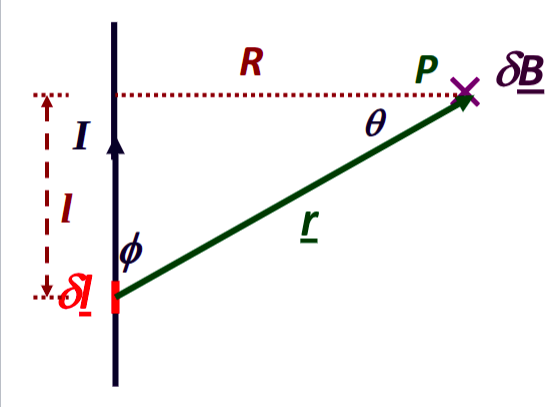
\includegraphics[width=0.75\textwidth]{figures/lec14-05.png}
     \caption{}
\end{figure}

We want to find the B-field from the lime of current. The B-field is going into the page at $P$, given by the cross. The Biot Savat Law again gives:
\[
    \delta \underline{B} = \frac{\mu_0 I}{4 \pi r^2} \delta \underline{L} \wedge \hat{r}
\]

As $\hat{r}$ is a unit vector, the magnitude is given with the magnitude of L and the sine of phi:
\[
    \delta B = \frac{\mu_0 I}{4 \pi r^2} \delta L \sin \phi \tag{1}
\]

We want this in terms of $\theta$ instead, and given these two angles form a right angled triangle we have:
\[
    \sin \phi = \sin \left(\frac{\pi}{2} - \theta\right) = \cos \theta \tag{2}
\]

Hence:
\[
    \delta B = \frac{\mu_0}{4 \pi r^2} \delta L \cos \theta
\]

By trig we simply have:
\[
    r \cos \theta = R \implies r = \frac{R}{\cos \theta} \tag{3}
\]
\[
    \tan \theta = \frac{L}{R} \implies L = R \tan \theta \implies \frac{dL}{d \theta} = \frac{R}{\cos^2 \theta}
\]
\[
    \implies \delta L = \frac{R}{\cos^2 \theta} \delta \theta \tag{4}
\]

Inserting (2), (3), (4) back into (1) gives:
\[
    \delta B = \frac{\mu_0 I}{4 \pi} \times \frac{\cos^2 \theta}{R^2} \times \cos \theta \times \frac{R}{\cos^2 \theta} \delta \theta
\]

Hence:
\[
    \delta B = \frac{\mu_0 I}{4 \pi} \frac{1}{R} \cos \theta \delta \theta
\]
\[
    B = \frac{\mu_0 I}{4 \pi R} \oint^{\theta_2}_{\theta_1} \cos \theta d \theta
\]

Where $\theta_1, \theta_2$ depend the angles given by the length of the wire.

\[
    \boxed{B = \frac{\mu_0 I}{4 \pi R} \left(\sin \theta_2 - \sin \theta_1\right)}
\]

If the wire was infinitely long, $\theta_2 = \pi/2$ and $\theta_1 = -\pi/2$ (technically a limit as  $L \to \infty$). This gives us:
\[
    B = \frac{\mu_0 I}{2 \pi R}
\]

\section{More Complex Loops}
Consider a current loop, with a set of axes centred at the middle of the loop. The loop sits in the $yz$ plane, and we step out some perpendicular distance $x$ in the $x$ plane.

\begin{figure}[H]
    \centering
    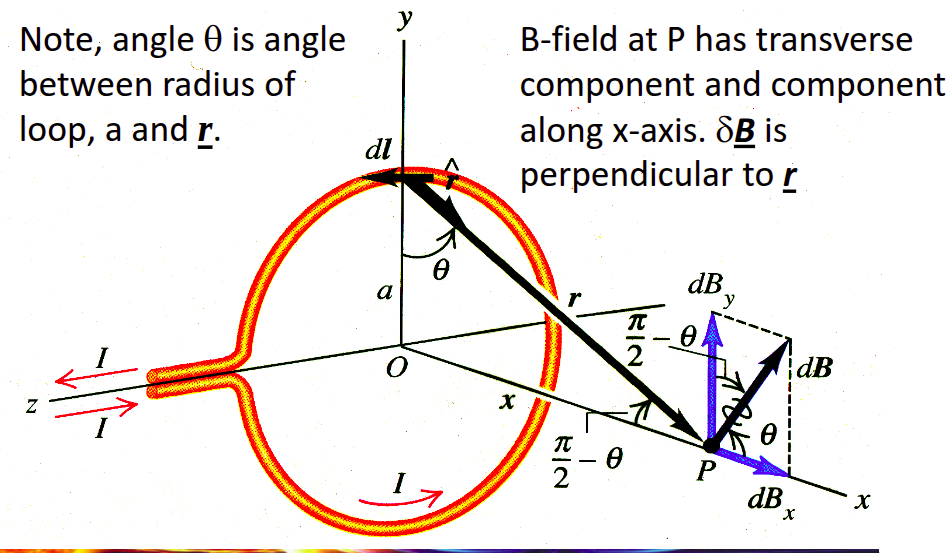
\includegraphics[width=0.75\textwidth]{figures/lec14-06.png}
     \caption{}
\end{figure}

We step some distance $\delta L$ along this loop, and the vector from the point we're investigating to B-field at from this $\delta L$ is $\underline{r}$, at angle $\theta$.

We can consider symmetry to see that transverse components to the axis will cancel each other out and therefore do not need considering:
\begin{figure}[H]
    \centering
    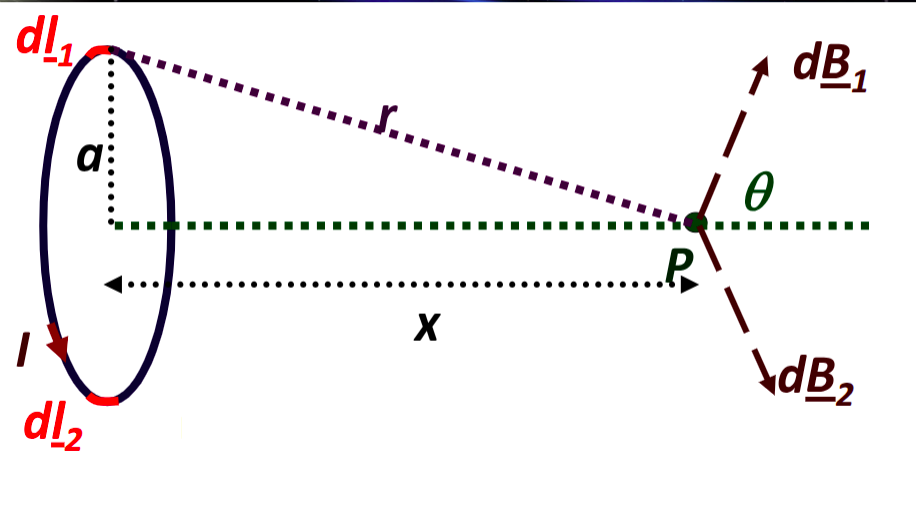
\includegraphics[width=0.75\textwidth]{figures/lec14-07.png}
     \caption{}
\end{figure}

Therefore all of the components of the B-field in the $yz$ planes will cancel out, and the only resultant B-field is in the x-direction. We will fully evaluate this on Monday.


